% \documentclass{article}
% \usepackage[utf8]{inputenc}
% \usepackage{fullpage}
% \usepackage{setspace}
% \usepackage[hang,flushmargin]{footmisc} %control footnote indent
% \usepackage{url} % for website links
% \usepackage{amssymb,amsmath}%for matrix
% \usepackage{graphicx}%for figure
% \usepackage{appendix}%for appendix
% \usepackage{float}
% \floatstyle{plaintop}
% \restylefloat{table}
% \usepackage{multirow}
% \usepackage{longtable}
% \usepackage{morefloats}%in case there are too many float tables and figures
% \usepackage{caption}
% \usepackage{subcaption}
% \usepackage{listings}
% \captionsetup[subtable]{font=normal}
% \usepackage{color}
% \usepackage{hyperref}
% \usepackage[round]{natbib}
% \usepackage{rotating} % rotate table by some degree
% \usepackage{rotfloat}



% %\usepackage{Sweave}
% \setlength{\parindent}{0em}
% \setlength{\parskip}{0.5em}


% \graphicspath{{0.plots/}}



% \begin{document}

%%%%%%%%%%%%%%%%%%%%%%%%%%%%%%%%%%%%%%%%%%%%%%%%%%%%%%%%
\subsection{Simulation Study} \label{sec:p3simulation}
%%%%%%%%%%%%%%%%%%%%%%%%%%%%%%%%%%%%%%%%%%%%%%%%%%%%%%%%
We conduct simulation studies to validate the proposed QRJM in making subject-specific dynamic predictions of future event-free probability. In the simulation studies, we assess the predicted event-free probability given in \eqref{eqn:pexpct_pred}, by comparing it with the ``gold standard'' calculated from the true (simulated) values of random effects, fixed effects, and other model parameters.

We simulate the data from Model (\ref{eqn:p3simjoint}), all the regression coefficients $\beta_1$, $\beta_2$, $\beta_3$, $\gamma$, and $\alpha$ are set to be 1. In the longitudinal process, we simulate $X_{1i}$ and the random effect $u_i$ from $N(0, 1)$, and $X_{2i}$ from $Bernuolli(0.5)$. A maximum of six observations are generated for each subject at follow-up times $t=0, 0.25, 0.5, 0.75, 1.0, \mbox{ and }1.25$. To simulate recurrent times, we set the baseline intensity $r_{0i}(t)$ to be constant 1 and generate $W_i$ from $N(0, 1)$. The random censoring time $C_i$ is generated from $2+Beta(1,1)$ and the recurrent times $T_{ik}^*$ are generated using calendar time. Finally, we set the observed recurrent times as $T_{ik} = min(C_i, T_{ik}^*)$ and recurrent event indicators as $\Delta_{ik} = I(T_{ik} < C_i)$ for $k=1, \cdots, m_i$. And we limit a maximum of five recurrent events for each subject.

\begin{equation}\label{eqn:p3simjoint}
\left\{
\begin{array}{l}
Y_{i}(t) = m_i(t) + \varepsilon_{i}(t) = \beta_1X_{1i} + \beta_2X_{2i} + \beta_3t + u_i + \varepsilon_{i}(t)\\
r_i(t|W_i;  \gamma, \alpha) = r_{0i}(t)\exp(\gamma W_i + \alpha m_i(t))
\end{array}
\right.
\end{equation}

We consider the following four scenarios in simulation study. For each scenario, we simulate 200 data sets with sample size equals to 500 in each. In the simulated data, around 90\% of the subjects have at least two events.
\begin{itemize}
\item Scenario 1: $\varepsilon_{i}(t)$ follows ALD with $\tau=0.25$ (right-skewed);
\item Scenario 2: $\varepsilon_{i}(t)$ follows ALD with $\tau=0.50$ (symmetric at 0, heavy tail);
\item Scenario 3: $\varepsilon_{i}(t)$ follows ALD with $\tau=0.75$ (left-skewed);
\item Scenario 4: $\varepsilon_{i}(t)$ follows standard normal distribution.
\end{itemize}

Before making predictions, 400 (80\%) out of the total 500 samples are randomly selected to draw model inference and the rest 100 subjects are used to make out-of-sample dynamic predictions of event-free probability. Inference results for all four scenarios can be found in Table~\ref{tab:p3sim_inference} in Appendices. From the results we can see in Scenarios 1 to 3, our Bayesian algorithm performs pretty well in recovering the true parameter values with small bias and MSE and high coverage probability. In Scenario 4, where the simulated data are normal, median regression (QRJM with $\tau=0.5$) also performs well and the result is comparable to the true model (not shown), thus QRJM is robust to model misspecification.

In the prediction part, we use the simulated data and true parameter values to calculate the event-free probability and use it as the ``gold standard''. To assess the prediction results from different models, we compare the predicted values with the gold standard in terms of bias and MSE. Bland-Altman plot \citep{bland1986statistical}, a commonly used method to compare the agreement of two measurement methods, is used to visualize the prediction results. To make the predictions ``dynamic'', we choose different combinations of follow-up time (i.e., $t$) and the prediction time interval (i.e., $\Delta t$) to mimic expected real-world scenario.

Table~\ref{tab:p3sim2qt25data} summarizes the prediction results from three follow-up time points ($t=$0.25, 0.50, and 1.00) combined with three prediction time window ($\Delta t$ = 0.25, 0.50, and 1.00) for Scenario 1. For fixed follow-up time $t$, with increasing prediction time window $\Delta t$, the accuracy and precision of the predicted values, compared with the gold standard, decrease gradually, i.e. large $\Delta t$ results in larger bias and MSE. This is expected due to increased uncertainty  in predictions for time points further into the future. When $\Delta t$ is fixed and follow-up time $t$ increases, we see improvement in the predictions, which is indicated by decreased MSE with longer follow-up time. This makes sense to us since with longer follow-up time we tend to have more longitudinal measurements as well as event data per subject. As a result, predictions become more precise with additional information from both outcomes. The same message can be found in the Bland-Altman plots. In Figure~\ref{plot:p3sim2qt25_true_pred}, as we fix the follow-up time $t$ and look horizontally, the variation of the plot increases. This is indicated by larger agreement intervals between the predictions and gold standard. While we fix the prediction time window $\Delta t$, the agreement becomes stronger with large follow-up time. Moreover, all Bland-Altman plots are horizontally spindle-shaped, suggesting that it is easier to predict a event-free probability near 0 or 1 than that near 0.5.

Comparing different models, Table~\ref{tab:p3sim2qt25data} also suggests that when data are generated from skewed distribution, the predictions from models other than the true model have larger MSE and bias thus are less reliable. When data are generated as normal, QRJM with $\tau=0.50$ performs comparably with the true model. In summary, the best predictions of event-free probability are obtained using the QRJM model and as expected, applying the exact quantile that generated the outcome data performs best and QRJM is robust to model misspecification. Additional simulation results can be found in Appendices Section~\ref{apped:p3_sim}.


\begin{table}[H]
\centering
\caption{Simulation study: MSE and bias of the difference between predicted event-free probability and the gold standard (Scenario 1).}
\adjustbox{max width=\textwidth}{
\label{tab:p3sim2qt25data}
\begin{tabular}{clcccccccc}
\hline
 & & \multicolumn{2}{c}{QRJM ($\tau=0.25$)} & &\multicolumn{2}{c}{QRJM ($\tau=0.5$)} & &\multicolumn{2}{c}{LMJM} \\
\cline{3-4}\cline{6-7}\cline{9-10}
$t$ & $\Delta t$ & MSE & Bias & & MSE & Bias & & MSE & Bias \\
\hline
\multirow{2}{*}{{\bf 0.25}} & 0.25 & 0.028 & 0.001 && 0.035 & 0.067 & & 0.033 & 0.023 \\
&  0.50 & 0.035 & $-$0.006 && 0.045 & 0.079 & & 0.043 & 0.024 \\
&  1.00 & 0.037 & $-$0.021 && 0.048 & 0.074 & & 0.046 & 0.015 \\
\hline
\multirow{2}{*}{{\bf 0.5}} & 0.25 & 0.022 & 0.002 && 0.029 & 0.067 & & 0.026 & 0.011 \\
&   0.50 & 0.029 & $-$0.005 && 0.039 & 0.078 & & 0.036 & 0.007 \\
&   1.00 & 0.033 & $-$0.018 && 0.043 & 0.077 & & 0.040 & $-$0.005\\
\hline
\multirow{2}{*}{{\bf 1.00}} & 0.25 & 0.018 & 0.011 && 0.025 & 0.078 & & 0.020 & 0.019 \\
& 0.50 & 0.023 & $-$0.005 && 0.033 & 0.079 & & 0.022 & $-$0.004  \\
&  1.00 & 0.026 & $-$0.016 && 0.036 & 0.078 & & 0.022 & $-$0.009\\
\hline
\end{tabular}
}
\end{table}

\begin{figure}[H]
\captionsetup[subfloat]{farskip=-5pt,captionskip=-1pt}
\centering
\subfloat[$t = $ 0.25]{
    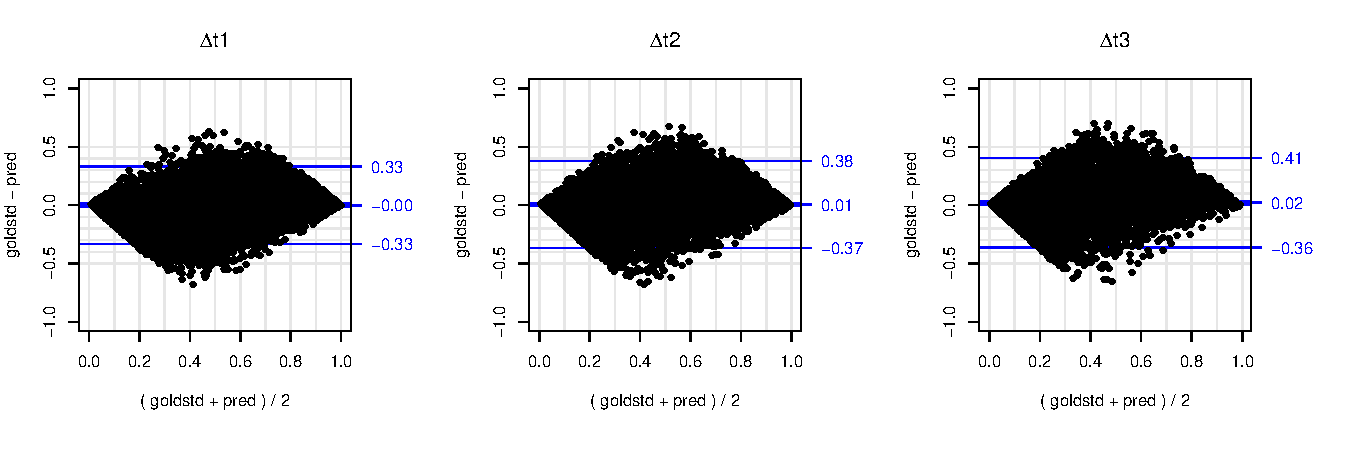
\includegraphics[width=\columnwidth]{p3_baplot_qt25data_qt25fit_t1.pdf}\label{plot:p3sim2fig121}
}

\centering
\subfloat[$t=$ 0.50]{
    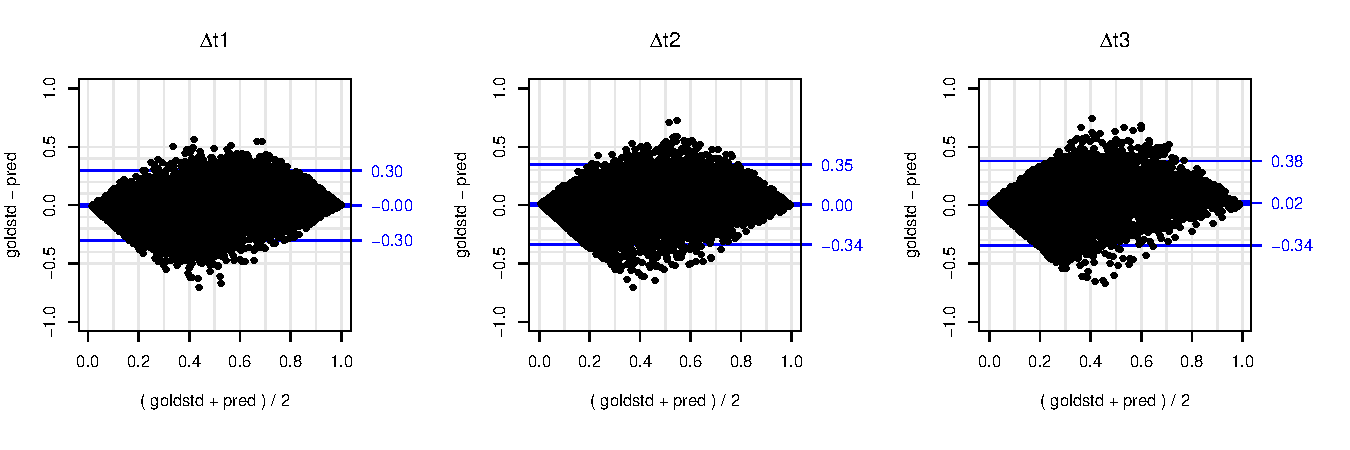
\includegraphics[width=\columnwidth]{p3_baplot_qt25data_qt25fit_t2.pdf}\label{plot:p3sim2fig122}
}

\centering
\subfloat[$t=$ 1.00]{
    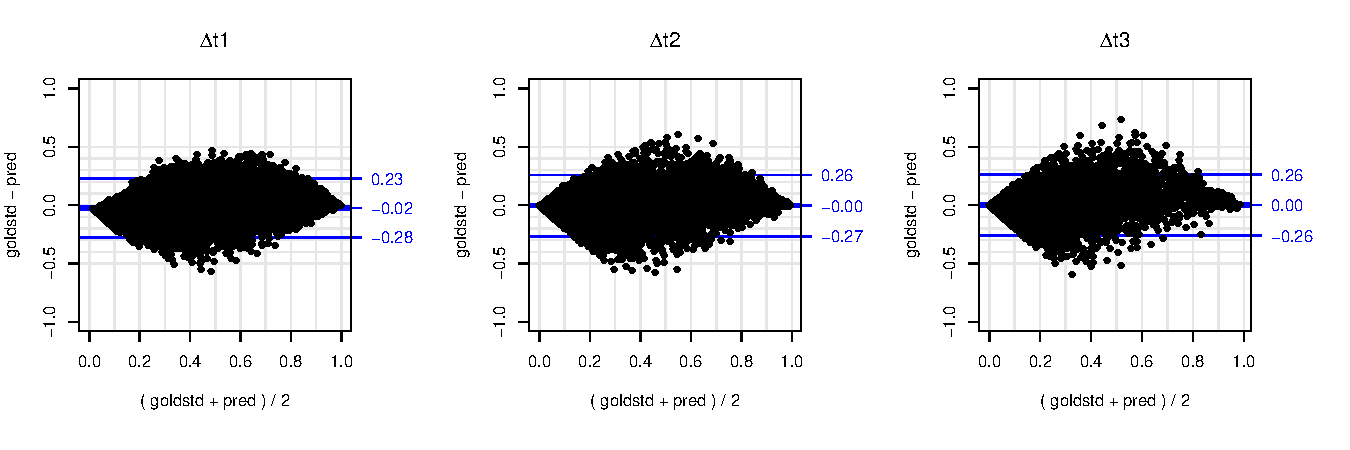
\includegraphics[width=\columnwidth]{p3_baplot_qt25data_qt25fit_t3.pdf}\label{plot:p3sim2fig123}
}
  \caption{Bland-Altman plot (bias and 95\% limits of agreement) of model predictions versus gold standard based on increasing follow-up time ($t$= 0.25, 0.50, and 1.00) and three different prediction time intervals ($\Delta t1 < \Delta t2 < \Delta t3$) under Scenario 1.}
  \label{plot:p3sim2qt25_true_pred}
\end{figure}


\begin{table}[H]
\centering
\caption{Simulation study: MSE and bias of the difference between predicted event-free probability and the gold standard (Scenario 4).}
\adjustbox{max width=\textwidth}{
\label{tab:p3sim2normdata}
\begin{tabular}{clccccc}
\hline
 & & \multicolumn{2}{c}{QRJM ($\tau=0.5$)} & &\multicolumn{2}{c}{LMJM}\\
\cline{3-4}\cline{6-7}
$t$ & $\Delta t$ & MSE & Bias & & MSE & Bias \\
\hline
\multirow{2}{*}{{\bf 0.25}} & 0.25 & 0.015 & $-$0.003 && 0.014 & $-$0.001 \\
&  0.50 & 0.019 & $-$0.007 &&  0.018 & $-$0.003 \\
&  1.00 & 0.020 & $-$0.014 && 0.019 & $-$0.010 \\
\hline
\multirow{2}{*}{{\bf 0.5}} & 0.25 & 0.012 & 0.001 && 0.011 & 0.002 \\
&   0.50 & 0.015 & $-$0.004 && 0.014 & $-$0.002\\
&   1.00 & 0.016 & $-$0.009 && 0.014 & $-$0.007 \\
\hline
\multirow{2}{*}{{\bf 1.00}} & 0.25 & 0.009 & 0.006 && 0.008 & 0.005 \\
& 0.50 & 0.010 & $-$0.004 && 0.009 & $-$0.003 \\
&  1.00 & 0.010 & $-$0.010 && 0.010 & $-$0.009 \\
\hline
\end{tabular}
}
\end{table}


%
%
%All is done in \LaTeX \cite{knuth1986texbook}.
%
%
% \bibliographystyle{plainnat}%%%%%%%%%%%%%%%%%%%%
% \addcontentsline{toc}{section}{References}
% \bibliography{QRJM}

% \end{document}